\documentclass[12pt,a4paper]{article}
\usepackage[utf8]{inputenc} % Input encoding for Chinese characters
\usepackage[T1]{fontenc} % Output font encoding
\usepackage{CJKutf8} % Chinese, Japanese, Korean support



%`\documentclass{article} \usepackage{xeCJK} \setCJKmainfont{SimSun} % Replace with your preferred Chinese font  \begin{document} This is some English text.  \begin{CJK*}{UTF8}{gbsn} 这是一些中文文本。 \end{CJK*}  More English text. \end{document}`


%In summary, \begin{CJK*} is more suitable when you need to ensure that CJK text does not break across lines or when you want precise control over spacing, but it may result in less flexible line-breaking. \begin{CJK} is more flexible, allowing automatic line-breaking and improved inter-character spacing for longer passages of CJK text within a document. The choice between them depends on your specific formatting requirements and preferences.




\usepackage[english]{babel} % Language setting (use 'chinese' for Chinese)
\usepackage{amsmath,amsfonts,amssymb} % Math packages
\usepackage{geometry} % Adjust page margins
\usepackage{enumitem} % Customize itemize/enumerate
\usepackage{fancyhdr} % Custom headers and footers
\usepackage{titlesec} % Customize section titles
\usepackage{graphicx} % Include images
\usepackage{hyperref} % Add hyperlinks
\usepackage{lipsum} % Dummy text for demonstration
\usepackage{lipsum}
\usepackage{fontspec}

% Page margins
\geometry{margin=1in}

\usepackage{makeidx}
\makeindex




%setmainfont{Helvetica Neue}

\bibliographystyle{IEEE}


% Custom headers and footers
\pagestyle{fancy}
\fancyhf{}
\rhead{Your Name}
\lhead{Lecture Notes}
\rfoot{Page \thepage}

% Customize section titles
\titleformat{\section}
{\normalfont\Large\bfseries}{\thesection}{1em}{}
\titleformat{\subsection}
{\normalfont\large\bfseries}{\thesubsection}{1em}{}

% Hyperlink settings
\hypersetup{
    colorlinks=true,
    linkcolor=blue,
    filecolor=magenta,
    urlcolor=cyan,
}


%%%%%%%%%%%%%%%%%%%%%%%%%%%%%%%%%%%%%%%%%%%%%%
 
%%%%%%%%%%%%%%%%%%%%%%%%%%%%%%%%%%%%%%%%%%%%%%%

%%%%%%%%%%%%%%%%%%%%%%%%%%%%%  A D D I T I O N A L   T O O L K I T %%%%%%%%%%%%%%%%%%%%%%%%%%%%

%%%%%%%%%%%%%%%%%%%%%%%%%%%%%%%%%%%%%%%%%%%%%%%%%%


%%%%%%%%%%%%%%%%%%%%%%%%%%%%%%%%%%%%%%%%%%%%%%
\usepackage{tocloft}  % Load the tocloft package for customization

\usepackage{tikz}

\usepackage{array}  % For customizing column formats
\usepackage{booktabs}  % For professional-looking tables
\usepackage{multirow}  % For multi-row cells


\usepackage{pgfplots}
%\pgfplotsset{compat=1.14}

%\usepackage{pgf-pie}



\usepackage{caption}   % For customizing captions





%%%%%%%%%%%%%%%%%%%%%%%%%%%%%%%%%%%%%%%%%%%%%%
 
%%%%%%%%%%%%%%%%%%%%%%%%%%%%%%%%%%%%%%%%%%%%%%%

%%%%%%%%%%%%%%%%%%%%%%%%%%%%%  A D D I T I O N A L   T O O L K I T  THE END %%%%%%%%%%%%%%%%%%%%%%%%%%%%

%%%%%%%%%%%%%%%%%%%%%%%%%%%%%%%%%%%%%%%%%%%%%%%%%%


%%%%%%%%%%%%%%%%%%%%%%%%%%%%%%%%%%%%%%%%%%%%%%




\begin{document}
\begin{CJK*}{UTF8}{gbsn} % Use the CJK package for Chinese text

\title{Chinese Version 1 Reading Notes}
\author{ChatGPT\footnote{August 3, 2020 version}, Your Name}
\date{\today}
\maketitle



\section{License}
This work is licensed under a Creative Commons \href{https://creativecommons.org/licenses/by-nc-sa/4.0/}{Attribution-NonCommercial-ShareAlike 4.0 International License}.

\section{Introduction}



\section{List of tables}

\listoffigures    % List of charts

\listoftables  % Add a list of tables

This is an \index{blurt} at the end of the day \index{amanda}.


\section{Tables}
\begin{table}[ht]
    \centering
    \caption{Sample Table}
    \label{tab:sample}
    \begin{tabular}{|c|c|c|}
        \hline
        \textbf{Column 1} & \textbf{Column 2} & \textbf{Column 3} \\
        \hline
        1 & A & \$100 \\
        \hline
        2 & B & \$200 \\
        3 & C & \$300 \\
        \hline
    \end{tabular}
\end{table}

\begin{minipage}{\linewidth}
\captionof{table}{Tabular Name} % Table name/label
\begin{tabular}{|c|c|c|}
    \hline
    \textbf{Header 1} & \textbf{Header 2} & \textbf{Header 3} \\
    \hline
    Row 1, Col 1 & Row 1, Col 2 & Row 1, Col 3 \\
    \hline
    Row 2, Col 1 & Row 2, Col 2 & Row 2, Col 3 \\
    \hline
    Row 3, Col 1 & Row 3, Col 2 & Row 3, Col 3 \\
    \hline
\end{tabular}
\end{minipage}

\section{graph table}
This is graph table
\clearpage  % Force figure to appear after the current section

\begin{table}[ht]
    \centering
    \caption{Graph Table}
    \label{tab:graph}
    \begin{tabular}{cccc}
        \toprule
        \textbf{Node} & \textbf{Connected to Node} \\
        \midrule
        A & B, C \\
        B & A, D \\
        C & A, D \\
        D & B, C \\
        \bottomrule
    \end{tabular}
\end{table}



\section{Column Charts}

This is Column Chart.


\begin{figure}[ht]
    \centering
    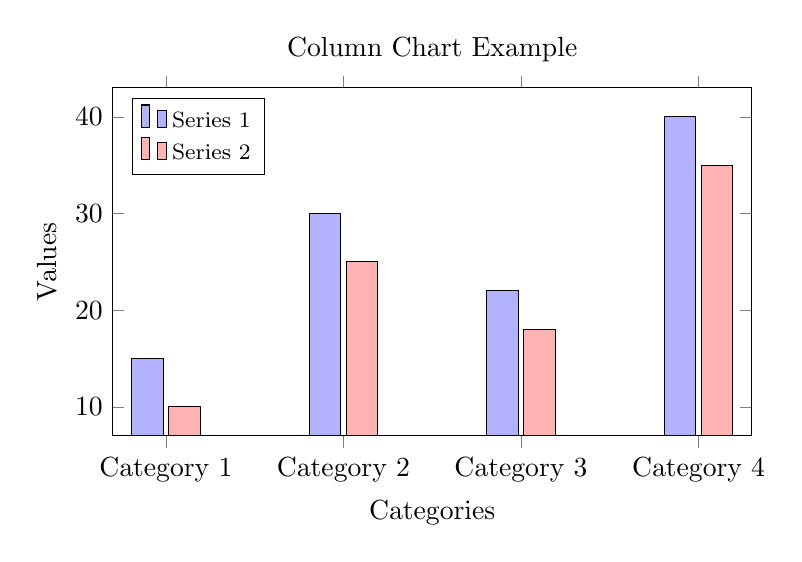
\begin{tikzpicture}
        \begin{axis}[
            ybar, % Vertical bars
            xlabel={Categories},
            ylabel={Values},
            symbolic x coords={Category 1, Category 2, Category 3, Category 4},
            xtick=data, % Use symbolic x coords as x-axis tick labels
            width=0.8\textwidth,
            height=6cm,
            bar width=0.4cm, % Width of the bars
            legend pos=north west, % Position of the legend
            legend style={font=\footnotesize},
            title={Column Chart Example},
        ]
        
        % Data series
        \addplot[fill=blue!30] coordinates {
            (Category 1, 15)
            (Category 2, 30)
            (Category 3, 22)
            (Category 4, 40)
        };
        
        \addplot[fill=red!30] coordinates {
            (Category 1, 10)
            (Category 2, 25)
            (Category 3, 18)
            (Category 4, 35)
        };
        
        \legend{Series 1, Series 2}
        
        \end{axis}
    \end{tikzpicture}
    \caption{Column Chart Example}
    \label{fig:column_chart}
\end{figure}

\section{Bar Charts}
This is bar chart. 
\clearpage  % Force figure to appear after the current section


\begin{figure}[ht]
    \centering
    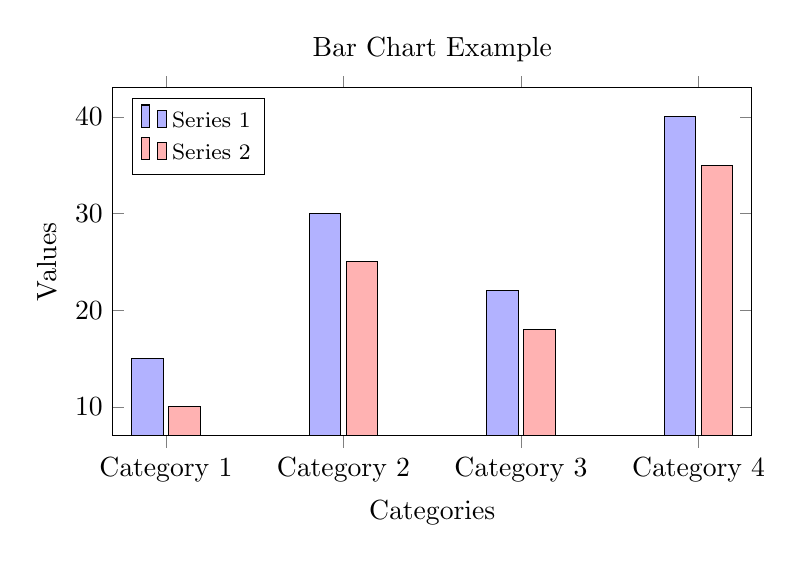
\begin{tikzpicture}
        \begin{axis}[
            ybar, % Vertical bars
            xlabel={Categories},
            ylabel={Values},
            symbolic x coords={Category 1, Category 2, Category 3, Category 4},
            xtick=data, % Use symbolic x coords as x-axis tick labels
            width=0.8\textwidth,
            height=6cm,
            bar width=0.4cm, % Width of the bars
            legend pos=north west, % Position of the legend
            legend style={font=\footnotesize},
            title={Bar Chart Example},
        ]
        
        % Data series
        \addplot[fill=blue!30] coordinates {
            (Category 1, 15)
            (Category 2, 30)
            (Category 3, 22)
            (Category 4, 40)
        };
        
        \addplot[fill=red!30] coordinates {
            (Category 1, 10)
            (Category 2, 25)
            (Category 3, 18)
            (Category 4, 35)
        };
        
        \legend{Series 1, Series 2}
        
        \end{axis}
    \end{tikzpicture}
    \caption{Bar Chart Example}
    \label{fig:bar_chart}
\end{figure}




\section{Line Chart}

This is line chart.
\clearpage  % Force figure to appear after the current section

\begin{figure}[ht]
    \centering
    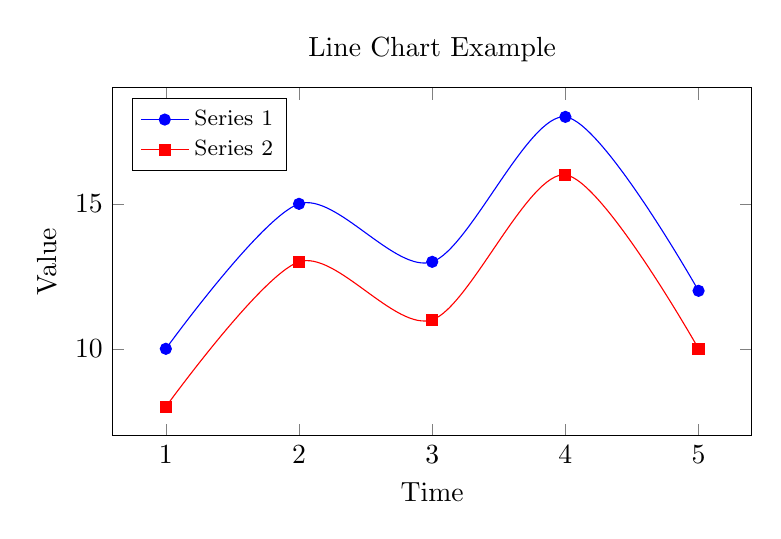
\begin{tikzpicture}
        \begin{axis}[
            xlabel={Time},
            ylabel={Value},
            width=0.8\textwidth,
            height=6cm,
            legend pos=north west, % Position of the legend
            legend style={font=\footnotesize},
            title={Line Chart Example},
        ]
        
        % Data series 1
        \addplot[blue,mark=*,smooth] coordinates {
            (1, 10)
            (2, 15)
            (3, 13)
            (4, 18)
            (5, 12)
        };
        \addlegendentry{Series 1}
        
        % Data series 2
        \addplot[red,mark=square*,smooth] coordinates {
            (1, 8)
            (2, 13)
            (3, 11)
            (4, 16)
            (5, 10)
        };
        \addlegendentry{Series 2}
        
        \end{axis}
    \end{tikzpicture}
    \caption{Line Chart Example}
    \label{fig:line_chart}
\end{figure}



\section{Spine Chart}

\clearpage

\begin{figure}
    \centering
    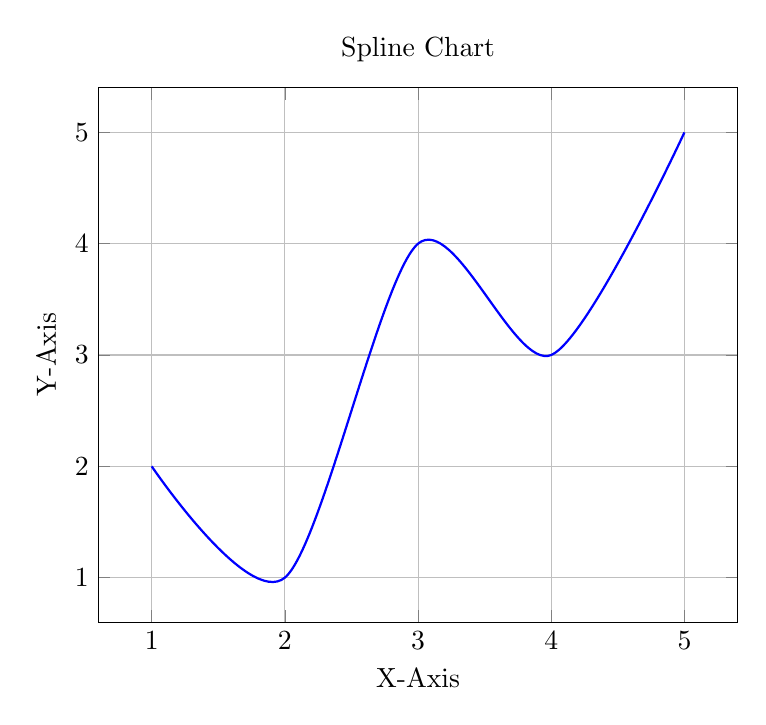
\begin{tikzpicture}
        \begin{axis}[
            width=0.8\textwidth,
            xlabel={X-Axis},
            ylabel={Y-Axis},
            title={Spline Chart},
            grid=major,
        ]
        
        % Sample data points
        \addplot+[smooth, mark=none, thick] coordinates {
            (1,2)
            (2,1)
            (3,4)
            (4,3)
            (5,5)
        };
        
        \end{axis}
    \end{tikzpicture}
    \caption{Spline Chart Example}
\end{figure}



\section{Area Chart}
\clearpage

\begin{figure}
    \centering
    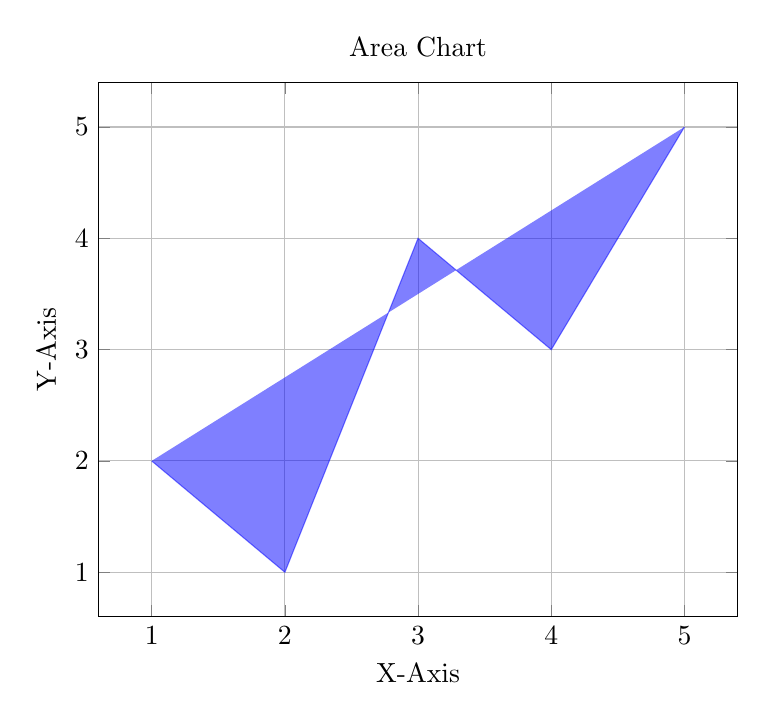
\begin{tikzpicture}
        \begin{axis}[
            width=0.8\textwidth,
            xlabel={X-Axis},
            ylabel={Y-Axis},
            title={Area Chart},
            grid=major,
        ]
        
        % Sample data points
        \addplot+[mark=none, fill=blue, opacity=0.5] coordinates {
            (1,2)
            (2,1)
            (3,4)
            (4,3)
            (5,5)
        };
        
        \end{axis}
    \end{tikzpicture}
    \caption{Area Chart Example}
\end{figure}





\section{Stacked}
\clearpage
\begin{figure}
    \centering
    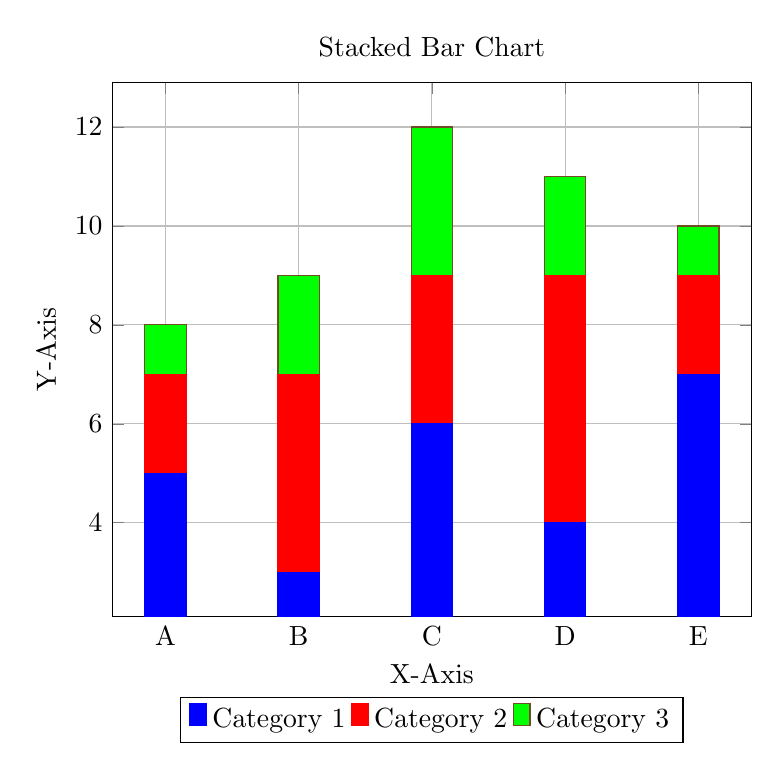
\begin{tikzpicture}
        \begin{axis}[
            width=0.8\textwidth,
            xlabel={X-Axis},
            ylabel={Y-Axis},
            title={Stacked Bar Chart},
            legend style={at={(0.5, -0.15)},
                anchor=north,legend columns=-1},
            ybar stacked,
            bar width=15pt,
            symbolic x coords={A, B, C, D, E},
            xtick=data,
            grid=major,
        ]
        
        % Sample data for each category
        \addplot+[fill=blue] coordinates {(A, 5) (B, 3) (C, 6) (D, 4) (E, 7)};
        \addplot+[fill=red] coordinates {(A, 2) (B, 4) (C, 3) (D, 5) (E, 2)};
        \addplot+[fill=green] coordinates {(A, 1) (B, 2) (C, 3) (D, 2) (E, 1)};
        
        \legend{Category 1, Category 2, Category 3}
        
        \end{axis}
    \end{tikzpicture}
    \caption{Stacked Bar Chart Example}
\end{figure}



\section{Combination chart}
\clearpage
\begin{figure}
    \centering
    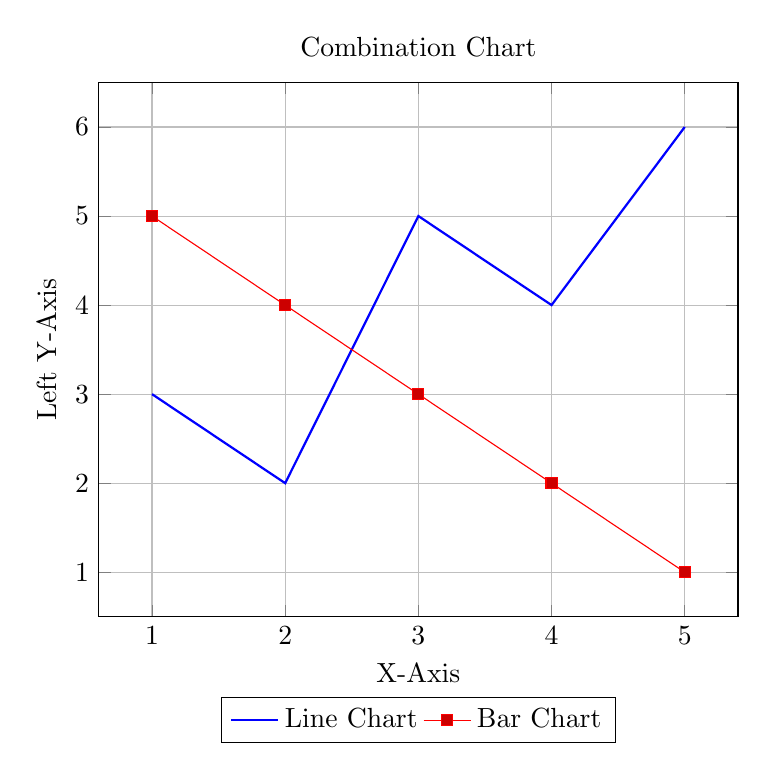
\begin{tikzpicture}
        \begin{axis}[
            width=0.8\textwidth,
            xlabel={X-Axis},
            ylabel={Left Y-Axis},
            title={Combination Chart},
            grid=major,
            legend style={at={(0.5,-0.15)},anchor=north,legend columns=-1},
        ]

        % Line chart
        \addplot+[blue,mark=none,thick] coordinates {
            (1,3)
            (2,2)
            (3,5)
            (4,4)
            (5,6)
        };
        \addlegendentry{Line Chart}
        
        % Bar chart
        \addplot+[red,fill=red!30,bar width=0.2] coordinates {
            (1,5)
            (2,4)
            (3,3)
            (4,2)
            (5,1)
        };
        \addlegendentry{Bar Chart}
        
        \end{axis}
    \end{tikzpicture}
    \caption{Combination Chart Example}
\end{figure}



\section{1}



\section{References}



\bibliography{main.bib}

\section{Index}

\printindex

\end{CJK*}
\end{document}
